\documentclass{beamer}

\title{Projet Graphes et Optimisation Combinatoire}
\author{Nicolas Vallois, Matilde Subtil, Virgil Surin, Simon Michel}
\institute{Université de Mons}
\date{20 décembre 2021}

\usetheme{Copenhagen}
\usepackage{verbatim}
\usepackage{graphicx}
\usepackage{mdwlist}
\usepackage{marvosym}
\usepackage{fancyvrb}
\usepackage{listings}
\usepackage[francais]{babel}

\begin{document}

\frame{\titlepage}


\begin{frame}
    \frametitle{Choix de la métaheuristique}
    3 méthodes sur lesquelles nous avons travaillé:
    \begin{itemize}
        \item Recherche locale
        \item Algorithme Evolutionnaire
        \item Recuit Simulé
    \end{itemize}

\end{frame}

\begin{frame}
    \frametitle{Méthodes rejetées}
    \begin{block}{Recherche Locale}
        Introduction au problème.
        Création d'une solution initiale aléatoire.
        Création d'un voisinage avec toutes les découpe possible (peu optimisé).\\~\\
        \MVRightarrow{} Mauvais résultats car on reste sur le minimum local (intensification pure)
    \end{block}
    
\end{frame}

\begin{frame}
    \frametitle{Méthodes rejetées}
    \begin{block}{Algorithme Évolutionnaire}
        Intention d'explorer au moins deux métaheuristiques afin de les comparer ou les combiner. \\~\\
        Étapes:
        \begin{itemize}
            \item Création d'une population aléatoire d'individus (solutions) 
            \item Sélection des parents par tournoi
            \item Croisement à un point 
            \item Hybridation par recherche locale
            \item Choix de la génération suivante par le meilleur coût.
        \end{itemize}
        Abandon au stade prototype car: peu de recherche sur les paramètres à utiliser en fonction du problème, mauvaise mise en place de la recherche locale et plus lent que le recuit quand on obtient des résultats similaires.
    \end{block}
\end{frame}

\begin{frame}[fragile]
    \frametitle{Méthodes rejetées}
    Recherche locale peu efficace basée sur des découpes équilibrées ! Ce qui empêche de trouver des voisins plus intéressants.
    \begin{exampleblock}{Paramètres}
        Taille population: 100, générations: 500\\
        Proba croisements: 0.85, proba hybridation: 0.01
    \begin{lstlisting}[basicstyle=\tiny]
        1 7660 5 1915 1915 1915 958 957
        2 7290 7 1042 1042 1042 1041 1041 1041 1041
        3 7040 4 1760 1760 1760 1760
        4 6890 4 1723 1723 1722 1722
        5 5860 3 1954 1953 1953
        6 5090 9 566 566 566 566 566 565 565 565 565
        7 4640 3 1791 1790 1059
        8 3830 2 1915 1915
        9 3460 2 1730 1730
        10 580 1 580
        B1 1954
        B2 1760
        B3 1059
        B4 580
        COST  5353
    \end{lstlisting}
    \end{exampleblock}
\end{frame}

\begin{frame}
    \frametitle{Motivation pour le choix du recuit simulé}
    Nous avons choisi le recuit simulé car il donnait de très bons résultats, tout en étant simple à implémenter.\\~\\

    L'adaptation de l'algorithme évolutionnaire demande beaucoup de fonctions à paramétrer qui impactent la solution: création de la population initiale, croisement qui peut rendre une solution indamissible(donc rééquilibrage nécessaire), recherche locale pour l'hybridation + paramètres.\\~\\

    Tandis que dans le recuit, il faut uniquement adapter les paramètres propres au recuit (températures, ...) et une fonction de création d'un voisin aléatoire.
\end{frame}

\begin{frame}
    \frametitle{Implémentation}
    Prototype en python pour une première implémentation du solveur.\\~\\

    Passage en C car plus rapide. Ajout de threads pour exécuter le recuit plusieurs fois en parallèle et garder la meilleure solution de ces recuits.

\end{frame}

\begin{frame}
    \frametitle{Choix d'un voisin}
    Pour choisir un voisin d'une solution: on choisit aléatoirement deux nombres i et j découpés de la solution. Ensuite on additionne le nombre de découpe et l'on divise ce nombre en deux d'une façon aléatoire: on obtient i\_split et j\_split.\\~\\
    Une fois qu'on a nos deux nombres de découpe, on doit choisir une méthode de découpe (voir slide suivant) qui travaille sur les données d'entrée i et j du problème en découpant i par i\_split et j par j\_split. 
\end{frame}

\begin{frame}
    \frametitle{Split Équilibré et Split Aléatoire}
    \begin{block}{Split Équilibré}
    Divise de façon équitable un entier x en n entiers.\\~\\
    \MVRightarrow{} Donne de bons résultats mais on peut faire encore mieux en éliminant la contrainte d'équilibre.
    \end{block}

    \begin{block}{Split Aléatoire}
    Divise de façon aléatoire un entier x en n entiers.\\~\\
    \MVRightarrow{} Donne parfois de très bons résultats mais aussi parfois de très mauvais. Il divise en trop petit nombres.
    \end{block}
\end{frame}

\begin{frame}[fragile]
    \frametitle{Exemples}
    \begin{exampleblock}{Split Équilibré - data1.dat}
        \begin{lstlisting}[basicstyle=\small]
        1 7660 4 1915 1915 1915 1915 
        2 7290 4 1823 1823 1822 1822 
        3 7040 4 1760 1760 1760 1760 
        4 6890 4 1723 1723 1722 1722 
        5 5860 9 652 651 651 651 651 651 651 651 651 
        6 5090 5 1018 1018 1018 1018 1018 
        7 4640 5 928 928 928 928 928 
        8 3830 2 1915 1915 
        9 3460 2 1730 1730 
        10 580 1 580 
        B1 1915
        B2 1760
        B3 1018
        B4 652
        COST 5345
        \end{lstlisting}
    \end{exampleblock}
\end{frame}

\begin{frame}[fragile]
    \frametitle{Exemples}
    \begin{exampleblock}{Split Aléatoire - Mauvais cas - data1.dat}
        \begin{lstlisting}[basicstyle=\small]
        1 7660 2 4017 3643 
        2 7290 6 4093 1434 1251 205 192 115 
        3 7040 6 4070 1413 1281 141 118 17 
        4 6890 3 4091 1418 1381 
        5 5860 6 3951 1313 177 161 154 104 
        6 5090 2 4043 1047 
        7 4640 2 3345 1295 
        8 3830 1 3830 
        9 3460 11 3447 2 2 2 1 1 1 1 1 1 1 
        10 580 1 580 
        B1 4093
        B2 1434
        B3 205
        B4 2
        COST 5734
        \end{lstlisting}
    \end{exampleblock}
\end{frame}

\begin{frame}[fragile]
    \frametitle{Exemples}
    \begin{exampleblock}{Split Aléatoire - Bon cas - data2.dat}
        \begin{lstlisting}[basicstyle=\tiny]
        1 9210 3 3136 3055 3019 
        2 9060 3 3071 3035 2954 
        3 8820 4 4285 2979 907 649 
        4 8350 2 4268 4082 
        5 7260 2 4213 3047 
        6 6950 2 3977 2973 
        7 5180 2 4272 908 
        8 4050 1 4050 
        9 3890 1 3890 
        10 3670 2 2888 782 
        11 3310 1 3310 
        12 3050 1 3050 
        13 2340 3 911 776 653 
        14 1790 2 912 878 
        15 930 1 930 
        B1 4285
        B2 3071
        B3 930
        COST 8286
        \end{lstlisting}
    \end{exampleblock}
\end{frame}

\begin{frame}
    \frametitle{Split Mix}
    Vu que chacun a un avantage dans certains cas, nous avons décidé de mélanger les deux méthode de Split. La façon dont ils sont mélangés se repose sur un paramètre "mix" qui défini la partie de x qui va dans le split équilibré et l'autre partie de x va dans le split aléatoire.
    On a que mix $\in [0,1]$. Si mix se rapproche de 0, la découpe sera plutôt aléatoire. Si mix se rapproche de 1, la découpe sera plutôt équilibrée. \\~\\

    On ne connait pas la bonne valeur de mix pour chaque problème, donc on fait tourner plusieurs threads en parallèles avec une valeur de mix qui augmente de façon linéaire entre chaque thread (ex: de 0 à 1 par pas de 0.25 si on a 5 threads).
\end{frame}

\begin{frame}[fragile]
    \frametitle{Exemples}
    \begin{exampleblock}{Split Mix - data2.dat}
        \begin{lstlisting}[basicstyle=\tiny]
        1 9210 3 4182 4126 902 
        2 9060 3 3078 2993 2989 
        3 8820 3 4006 3917 897 
        4 8350 2 4179 4171 
        5 7260 2 4182 3078 
        6 6950 2 4162 2788 
        7 5180 2 2734 2446 
        8 4050 1 4050 
        9 3890 1 3890 
        10 3670 2 2891 779 
        11 3310 2 2896 414 
        12 3050 1 3050 
        13 2340 3 924 878 538 
        14 1790 2 927 863 
        15 930 1 930 
        B1 4182
        B2 3078
        B3 930
        COST 8190
        \end{lstlisting}
    \end{exampleblock}
\end{frame}

\begin{frame}
    \frametitle{Choix des paramètres du recuit}
    Nous avons plusieurs paramètres
    \begin{itemize}
    \item La température initiale: elle ne doit pas être trop élevée sinon le début de la recherche sera dans une diversification pure.
    \item La température finale: elle ne doit pas être trop basse sinon on passe la fin de la recherche dans une intensification pure.
    \item Difficulté: déterminer les bonnes valeurs pour éviter de perdre du temps dans la diversification et intensification pure.
    \item Le coefficient de décroissance de la tempéature: compris entre 0 et 1. On a choisit 0.95 pour avoir une décroissance "douce".
    \item Le palier: plus la valeur est élevée, plus la recherche dure longtemps mais on trouve de meilleurs solution.
    \end{itemize}

\end{frame}

\begin{frame}
    \frametitle{Illustration de la recherche}
    \begin{figure}
        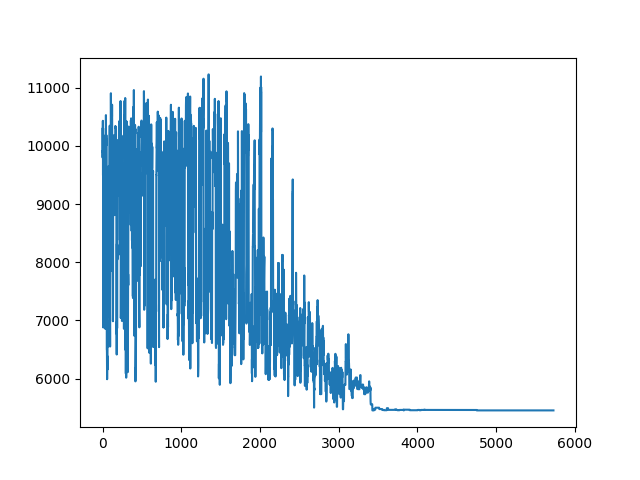
\includegraphics[width=\linewidth]{Figure_1.png}
        \caption{Stabilisation d'une recherche sur une solution}
    \end{figure}
\end{frame}


\begin{frame}
    \frametitle{Résultats obtenus}
    %Temp 100 temp finale: 0.01  threads 12 decreasing
    \begin{block}{Paramètres}
    Température intiale: 100, Température finale: 0.01 \\
    Coefficient de décroissance : 0.99, steps: 5000, Threads: 32
    \\~\\
        \centering
        \begin{tabular}{|c|c|c|c|c|}
            \hline
            fichier & solution & référence & différence & \% \\
            \hline
            \hline
            data1.dat & 5345 & 5243 & +102 & +1.945451 \\
            data2.dat & 8190 & 8190 & 0 & 0.000000 \\
            data3.dat & 3967 & 3897 & +70 & +1.796254 \\  
            data4.dat & 10092 & 9978 & +114 & +1.142514 \\ 
            data5.dat & 5064 & 4966 & +98 & +1.973419 \\  
            data6.dat & 15040 & 15030 & +10 & +0.066534 \\
            data7.dat & 7271 & 7194 & +77 & +1.070336 \\
            data8.dat & 239162 & 239778 & -616 & -0.256904 \\
            data9.dat & 230055 & 229428 & +627 & +0.273288 \\
            data10.dat & 229182 & 226788 & +2394 & +1.055611 \\
            \hline
        \end{tabular}
    \end{block}
    
\end{frame}

\begin{frame}
    \frametitle{Conclusion}
    Avec le recuit simulé, on arrive à avoir des solutions plutôt bonnes. Nous avons pu mettre en place la recherche d'un voisin suite à deux observations, en combinant nos méthodes. Évidemment, on peut toujours trouver mieux.  \\~\\
    Il est également dommage d'avoir arrêté de développer l'algorithme évolutionnaire car avec une meilleure recherche locale, il aurait peut-être donné de meilleur résultat que ce qui a été trouvé. 
\end{frame}

\end{document}